\documentclass{article}
\usepackage{ctex}
\usepackage{amsmath}
\usepackage{amssymb}
\usepackage{amsthm}
\usepackage{amsfonts}
\usepackage{physics}
\usepackage{geometry}
\usepackage{graphicx}
\usepackage{pgfplots}
\pgfplotsset{compat=1.18}
\usepackage{tikz-feynman}
\usepackage{caption}
\usepackage{subcaption}
\usepackage{hyperref}
\usepackage{float}
\usepackage{fancyhdr}

\pagestyle{fancy}
\fancyhead[L]{
    \begin{minipage}[c]{0.06\textwidth}
        \centering
        
\includegraphics[height=7.5mm]{院徽.jpg}
    \end{minipage}
    \begin{minipage}[c]{0.4\textwidth}
    The Note of Quantum Field Theory
    \end{minipage}
}
\fancyfoot[C]{\thepage}

%\setlength{\textwidth}{1.2\textwidth}
%\setlength{\textheight}{0.8\textheight}

\newtheorem{theorem}{定理}
\newtheorem{definition}{定义}
\newtheorem{example}{例}
\newtheorem{solution}{解}
\newtheorem{question}{题目}



\geometry{
paper = a4paper,    %纸张类型
top = 3cm,          %上页边距
bottom = 3cm,       %下页边距
left = 3cm,         %左页边距
right = 3cm         %右页边距
}

\newcommand{\ds}{\displaystyle}
\newcommand{\bb}[1]{\mathbb{#1}}
\newcommand{\h}[1]{\hat{#1}}
\newcommand{\pmtwo}[4]{\begin{pmatrix}#1&#2\\#3&#4\end{pmatrix}}
\newcommand{\pmthree}[9]{
    \begin{pmatrix}
        #1&#2&#3\\
        #4&#5&#6\\
        #7&#8&#9
    \end{pmatrix}
}
\newcommand{\vmtwo}[4]{\begin{vmatrix}#1&#2\\#3&#4\end{vmatrix}}
\newcommand{\vmthree}[9]{
    \begin{vmatrix}
        #1&#2&#3\\
        #4&#5&#6\\
        #7&#8&#9
    \end{vmatrix}
}

\newcommand{\vmthreedot}[9]{
    \begin{vmatrix}
        #1&#2&\cdots&#3\\
        #4&#5&\cdots&#6\\
        \vdots&\vdots&\ddots&\vdots\\
        #7&#8&\cdots&#9
    \end{vmatrix}
}

\newcommand{\expectation}[1]{\langle #1 \rangle}

\newcommand{\Da}[2]{\frac{\partial}{\partial#2}#1}

\newcommand{\D}[2]{\frac{d}{d#2}#1}

\newcommand{\id}[1]{\ket{#1}\bra{#1}}





\title{Note of QFT}
\author{Kaiser\\University of South China}








\begin{document}

\maketitle

\begin{abstract}
    \normalsize
    这一篇笔记是自己为了扩充自己的眼界以及学习更多的内容所准备的,同时也是为了在组会当中进行汇报而打的一个“小抄”
\end{abstract}

\begin{center}
    \large
    \begin{thebibliography}{99} 
        \bibitem{1} David Tong,\textit{Quantum Field Theory}
        \bibitem{2} M.Peskin and D.Schroeder,\textit{An Introduction of Quantum Field Theory}
        \bibitem{3} A.Zee,\textit{Quantum Field Theory in a Nutshell}
        \bibitem{4} S.Weinberg,\textit{The Quantum Theory of Field (Volume 1)}
        \bibitem{5} Landau,Lev D.,and Lifshitz,E.M.,\textit{The Classical Theory of Field}
        \bibitem{6} 高显,\textit{经典力学}
        \bibitem{7} 陈童,\textit{经典场论}
        \bibitem{8} 埃格先生,\textit{微分流形与分析力学初步}
        \bibitem{9} 陈童,\textit{经典力学新讲}
        \bibitem{10} Tom Lancaster,Stephen J.Blundell,\textit{Quantum Field Theory For Gifted Amature}
    \end{thebibliography}
\end{center}




\begin{center}
    \tableofcontents
\end{center}
\newpage





\section{经典力学与狭义相对论复习}

\subsection{伽利略变换}
考虑两个沿着$x$轴方向相对运动的惯性观察者,在$t=0$时,两者是互相重合的,并且我们假设它们之间的相对运动的速度(即相对速度)为常数,他们将会分别对应到两个参考系$S$和$S^\prime$,我们可以给出它们此时之间的坐标变换关系:
\begin{align*}
    S\to S^\prime:
    \begin{cases}
        &t^\prime=t\\
        &x^\prime=x-vt\\
        &y^\prime=y\\
        &z^\prime=z
    \end{cases}
\end{align*}

我们将其使用矩阵语言来进行表示就是:
\begin{align*}
    \begin{pmatrix}
        t^\prime\\x^\prime\\y^\prime\\z^\prime
    \end{pmatrix}
    =
    \begin{pmatrix}
        1&0&0&0\\
        -v&1&0&0\\
        0&0&1&0\\
        0&0&0&1
    \end{pmatrix}
    \begin{pmatrix}
        t\\x\\y\\z
    \end{pmatrix}
\end{align*}

同时,值得注意的是,我们连续地做两次伽利略变换得到的还会是伽利略变换,对于任意一个伽利略变换也都存在一个逆变换(将速度从$v$改成$-v$即可),当$v=0$时的伽利略变换将会是一个恒等变换,当然,伽利略变换也满足结合律,这也就是说,伽利略变换在数学上是构成了一个群的,并且,由于该群的变换参数$v$是一个可以连续变化的,因此他将对应着一个连续群(李群)的数学结构,叫作“伽利略变换群”,并且,容易发现,经典力学中的牛顿运动定律
\begin{align*}
    \vec{F}=m\vec{a}=m\frac{d^2}{dt^2}\vec{x}
\end{align*}

在伽利略变换下可以保持数学形式不变,用现代理论物理的语言来说,这意味着伽利略变换时牛顿运动定律的一个对称性,但是,其所导出的速度的相对关系为
\begin{align*}
    u^\prime&=\frac{d x^\prime}{dt^\prime}\\
    &=\frac{d(x-vt)}{dt}\\
    &=u-v
\end{align*}

很显然,这是非常符合日常生活经验和直觉的,直到迈克尔逊莫雷实验的出现,告诉我们,\textbf{真空中光速不变},但是很显然,伽利略


\subsection{经典力学}
写这一部分的内容,主要是为了让接下来在讲解经典力学以及经典场论时都有一定的物理基础,并且明白,为什么我们的拉格朗日力学所研究的空间是位形空间,需要的是广义坐标$q$,广义速度$\dot{q}$,而哈密顿力学研究的是相空间,使用的是正则坐标$q$,正则动量$p$。在搞明白了这些之后,我们才能真正的理解经典力学,并且向着经典场论靠近。
\subsubsection{位形、位形空间、广义坐标、广义速度}




\subsubsection{相空间、正则坐标、正则动量}
































\section{经典场论}
有一定的量子场论基础的人都知道,即使没有经典场论的基础(或者说是没有经典连续场的基础)也是无伤大雅的,因为量子场可以不依赖于经典连续场引入,但是就我个人认为,学习和重温量子场论中的基本概念以及很多的处理方法是必要的。同时,从经典场出发进行量子化得到粗糙的量子场,再根据其存在的漏洞进行正规化、重整化以获得具有预言能力的量子场论。

在这一部分,或者说这一次汇报中,我将讨论经典场论的几个方面。



\subsection{场算符(Field operators)}

\subsubsection{坐标与动量表象}
在此之前我们先回顾一下量子力学我们在描述一个态 $\ket{\alpha}$ 时可以使用坐标来描述 $\psi_\alpha(\vec{x}) = \braket{\vec{x}}{\alpha}$ 或者是用动量来描述 $\tilde{\psi}_\alpha(\vec{p}) = \braket{\vec{p}}{\alpha}$ 
\begin{equation*}
    \braket{\vec{p}}{\alpha} = \int d^3 x \braket{\vec{p}}{\vec{x}}\braket{\vec{x}}{\alpha}
\end{equation*}

接着在使用傅里叶变换
\begin{equation*}
    \tilde{\psi}_\alpha (\vec{p}) = \frac{1}{\sqrt{\mathcal{V}}} \int d^3 x e^{-i\vec{p}\cdot \vec{x}} \psi_\alpha (\vec{x})
\end{equation*}

因此 
\begin{equation*}
    \braket{\vec{p}}{\vec{x}} = \frac{1}{\sqrt{\mathcal{V}}} e^{-i\vec{p} \cdot \vec{x}}
\end{equation*}

如果 $\vec{p}$ 是离散的值时,其逆变换为
\begin{equation*}
    \psi_\alpha (\vec{x}) = \frac{1}{\sqrt{\mathcal{V}}} \sum_{\vec{p}} e^{i\vec{p}\cdot \vec{x}} \tilde{\psi}_\alpha (\vec{p})
\end{equation*}


\subsubsection{简单谐振子(Simple harmonic oscillators)}
接下来回顾一下简单谐振子问题,其势能为 $\displaystyle \hat{V} = \frac{1}{2} K \hat{x}^2$ ,通过求解其薛定谔方程可以得到波函数
\begin{equation*}
    \psi_n(\xi) = \frac{1}{\sqrt{2^n n!}}\left(\frac{m\omega}{\pi \hbar}\right)^{1/4} H_n(\xi) e^{\frac{1}{2}\xi^2} ,\qquad \xi = \sqrt{\frac{m\omega}{\hbar}}x
\end{equation*}

其中的 $\displaystyle H_n(\xi)$ 为厄密多项式,这里给出几幅波函数的图像
\begin{figure}[hbpt]
    \begin{minipage}{0.45\textwidth}
        \centering
        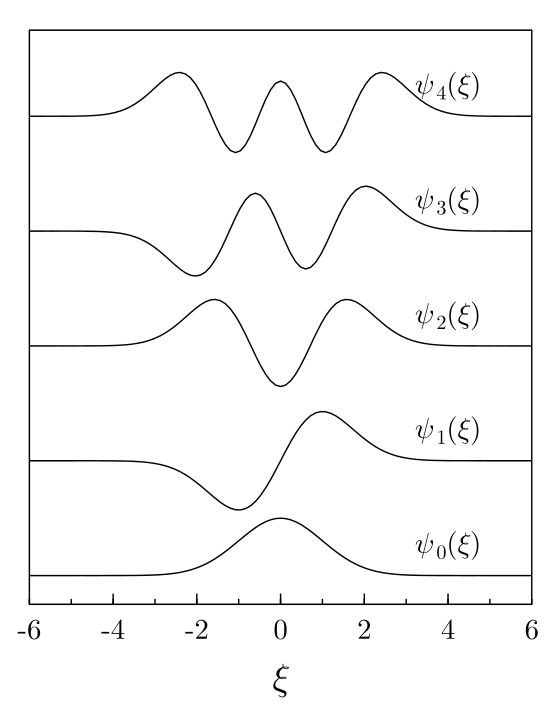
\includegraphics[width = 0.8\textwidth]{figure/一维简单谐振子解.png}
    \end{minipage}
    \hfill
    \begin{minipage}{0.45\textwidth}
        \centering
        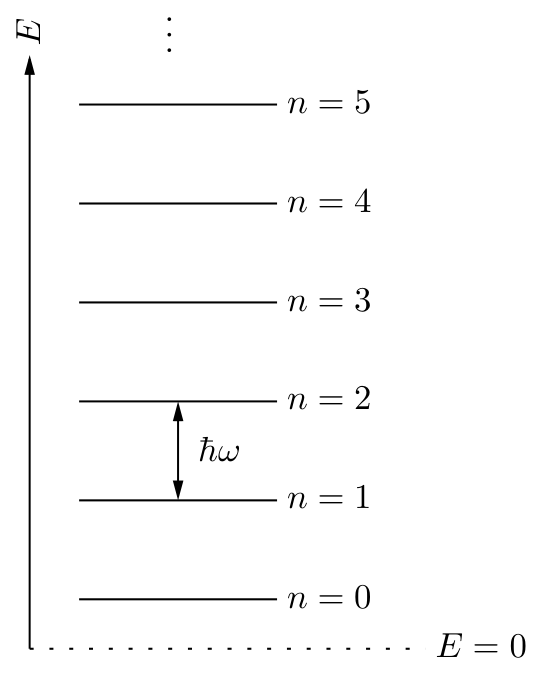
\includegraphics[width = 0.8\textwidth]{figure/一维简单谐振子能谱.png}
    \end{minipage}
\end{figure}

同时,其能谱(能量本征值)为 
\begin{equation*}
    E_n = \left(n + \frac{1}{2}\right)\hbar\omega
\end{equation*}

另外在求解过程当中我们还得到了一个所谓的频率 $\omega$ 并且将原来的常数 $K$ 进行了定义 $K\equiv m\omega^2$,于是哈密顿量重写为
\begin{equation*}
    \hat{H} = \frac{\hat{p}^2}{2m} + \frac{1}{2} m \omega^2 \hat{x}^2
\end{equation*}

似乎我们可以根据平方差写成这样的形式
\begin{equation*}
    \frac{1}{2} m \omega^2\left(\hat{x} - \frac{i}{m\omega}\hat{p}\right)\left(\hat{x} + \frac{i}{m\omega}\hat{p}\right)
\end{equation*}

但是将其展开所得到的为
\begin{equation*}
    \frac{\hat{p}^2}{2m} + \frac{1}{2} m \omega^2 \hat{x}^2 - \frac{1}{2}\hbar\omega = \hat{H} - \frac{1}{2}\hbar\omega
\end{equation*}

这相差的 $\displaystyle \frac{1}{2}\hbar\omega $ 是由于要修正零点能

在这里,算符 $\hat{x},\hat{p}$ 是厄密的,而算符 $\displaystyle \hat{x} - \frac{i}{m\omega}\hat{p}$ 与算符 $\displaystyle \hat{x} + \frac{i}{m\omega}\hat{p}$ 是互相自伴的,这也导致这两个新的算符是非厄密的,因此无法将其联系到任何的可观测量,我们给这两个算符进行重新定义,得到了所谓的产生和湮灭算符 $\hat{a}^\dagger,\hat{a}$
\begin{align*}
    \hat{a}^\dagger = \sqrt{\frac{m\omega}{2\hbar}}\left(\hat{x} - \frac{i}{m\omega}\hat{p}\right) \\
    \hat{a} = \sqrt{\frac{m\omega}{2\hbar}}\left(\hat{x} + \frac{i}{m\omega}\hat{p}\right)
\end{align*}

通过计算我们可以得到以下几个关系式
\begin{align*}
    \left[\hat{a},\hat{a}^\dagger\right] &= 1 \\
    \hat{x} &= \sqrt{\frac{\hbar}{2m\omega}} \left(\hat{a} + \hat{a}^\dagger\right) \\
    \hat{p} &= -i\sqrt{\frac{\hbar m \omega}{2}} \left(\hat{a} - \hat{a}^\dagger\right) \\
    \hat{H} &= \hbar \omega \left(\hat{a}^\dagger \hat{a} + \frac{1}{2}\right)
\end{align*}


如果我们设算符 $\hat{a}^\dagger \hat{a}$ 有本征值为 $n$ 的本征态 $\ket{n}$ 那么相应的谐振子的哈密顿量也会有相应的本征值为 $\hbar \omega \left(\frac{1}{2} + n\right)$ 的本征态 $\ket{n}$ 这刚刚好和我们算到的能量本征值 $E_n = \hbar \omega \left(\frac{1}{2} + n\right)$ 对应上,接下来我们只需要证明一下 $n$ 取非零整数即可,关于其非负性容易证明
\begin{equation*}
    n = \bra{n}\hat{a}^\dagger\hat{a}\ket{n} = \left|\hat{a}\ket{n}\right|^2 \geqslant  0
\end{equation*}


\subsubsection{占有数表象(Occupation number representation)}

在这里为了方便起见,我们用别的符号来定义一下这个算符,并且命名为粒子数算符(number operator)
\begin{equation*}
    \hat{n} = \hat{a}^\dagger \hat{a}
\end{equation*}


这样就有
\begin{equation*}
    \hat{n}\ket{n} = n\ket{n}
\end{equation*}


然后就是这些关系,这里不做证明,证明很简单,大家可以自己尝试一下
\begin{align*}
    \hat{n}\hat{a}^\dagger\ket{n} &= \left(n + 1\right) \ket{n} \\
    \hat{n}\hat{a}\ket{n} &= \left(n - 1\right) \ket{n} \\
    \hat{a}^\dagger \ket{n} &= \sqrt{n + 1}\ket{n + 1} \\
    \hat{a} \ket{n} &= \sqrt{n} \ket{n}
\end{align*}

很显然,我们的湮灭算符 $\hat{a}$ 可以使简单谐振子的能级下降一级,而我们的产生算符 $\hat{a}^\dagger$ 可以使简单谐振子的能级增加一级,因此如果我们不断地对一个本征态 $\ket{n}$ 作用上湮灭算符 $\hat{a}$ ,那么最终将会降到基态(真空态)$\ket{0}$ ,在这里我们规定:当湮灭算符作用到基态时,为 $0$,即 $\displaystyle \hat{a}\ket{0} = 0$,在这个规定下,我们的哈密顿量在基态的能量本征值为
\begin{equation*}
    \hat{H} \ket{0} = \hbar\omega \left(\hat{n} + \frac{1}{2}\right) \ket{0} = \frac{1}{2}\hbar\omega \ket{0}
\end{equation*}

可以看到这时候的基态就是我们的零点能。

另外,我们也可以不断地对某个态作用上产生算符 $\hat{a}^\dagger$ ,最终我们可以得到第 $n$ 能级的态矢量
\begin{equation*}
    \ket{n} = \frac{\left(\hat{a}^\dagger\right)^n}{\sqrt{n!}}\ket{0}
\end{equation*}

接下来考虑更为一般的情况,哈密顿量为很多独立的哈密顿量的总和
\begin{equation*}
    \hat{H} = \sum_{k = 1}^{N} \hat{H}_k =\sum_{k = 1}^{N} \left(\frac{\hat{p}_k^2}{2m_k} + \frac{1}{2} m_k \omega_k^2 \hat{x}_k^2\right)
\end{equation*}

我们将此时的态矢量记作每一个能级上的粒子数量的个数,例如
\begin{equation*}
    \ket{n_1,n_2,\cdots,n_k,\cdots}
\end{equation*}

当我们的产生湮灭算符作用到这些态上时将会是这样的效果
\begin{align*}
    \hat{a}_k^\dagger \ket{n_1,n_2,\cdots,n_k,\cdots} &\propto \ket{n_1,n_2,\cdots,n_k + 1,\cdots} \\
    \hat{a}_k \ket{n_1,n_2,\cdots,n_k,\cdots} &\propto \ket{n_1,n_2,\cdots,n_k - 1,\cdots}
\end{align*}

而对于这些升降算符有这样的对易关系
\begin{align*}
    \left[\hat{a}_k,\hat{a}_q\right] &= \left[\hat{a}_k^\dagger,\hat{a}_q^\dagger\right] = 0 \\
    \left[\hat{a}_k,\hat{a}_q^\dagger\right] &= \delta _{kq}
\end{align*}

此时的哈密顿量也可以像之前的简单谐振子问题一样,写成
\begin{equation*}
    \hat{H} = \sum_{k=1}^{N} \hbar\omega_k \left(\hat{a}_k^\dagger \hat{a}_k + \frac{1}{2}\right)
\end{equation*}

同时我们定义真空态(基态)为 $\displaystyle \ket{0,0,0,\cdots}$,也同样有
\begin{equation*}
    \hat{a}_k \ket{0,0,0,\cdots} = 0
\end{equation*}

而产生算符也有和简单谐振子的相似性质
\begin{equation*}
    \ket{n_1,n_2,\cdots,n_N} = \frac{1}{\sqrt{n_1! n_2! \cdots n_N!}}\left(\hat{a}_1^\dagger\right)^{n_1}\left(\hat{a}_2^\dagger\right)^{n_2}\cdots\left(\hat{a}_N^\dagger\right)^{n_N} \ket{0,0,0,\cdots}
\end{equation*}

简单记作
\begin{equation*}
    \ket{\left\{n_k\right\}} = \prod_k \frac{1}{\sqrt{n_k!}}\left(\hat{a}_k^\dagger\right)^{n_k}\ket{0}
\end{equation*}

在这里,我们所讨论的其实一直是在谐振子背景下产生量子,但不应该仅仅只在谐振子问题下,还应该让粒子在一个特定的动量态(momentum state) $\ket{p_m}$ ,因此我们将下标 $k$ 改为下标 $p_m$ 以此来表示在特定的 momentum state 下的算符,但是这一步操作仍然需要很谨慎的进行,接下来举个例子

\begin{example}
    给定一个双粒子体系其 momentum states 分别为 $p_1,p_2$ ,那么在 Occupation number representation 下,态矢量表示为 $\ket{n_1,n_2}$,我们做如下定义
    \begin{equation*}
        \hat{a}_{p_1}^\dagger \ket{00} = \ket{10} ,\quad \hat{a}_{p_2}^\dagger \ket{00} = \ket{01}
    \end{equation*}

    根据这个定义,我们有 
    \begin{equation*}
        \hat{a}_{p_2}^\dagger\hat{p_1}^\dagger \ket{0} \propto \ket{11} ,\quad \hat{a}_{p_1}^\dagger\hat{p_2}^\dagger \ket{0} \propto \ket{11}
    \end{equation*}

    这也就是说 
    \begin{equation*}
        \hat{a}_{p_2}^\dagger\hat{p_1}^\dagger = \lambda \hat{a}_{p_1}^\dagger\hat{p_2}^\dagger
    \end{equation*}

    在这里,我们假设 $\lambda = \pm 1$ 至于别的情况我们之后再说,这里的假设将会导致波函数出现对称和反对称两种情况
    \begin{enumerate}
        \item[case 1] $\lambda = 1$ ,我们将这时候的粒子称为玻色子
        \begin{equation*}
            \hat{a}_{p_2}^\dagger\hat{p_1}^\dagger = \hat{a}_{p_1}^\dagger\hat{p_2}^\dagger
        \end{equation*}

        根据这个式子我们知道对易关系
        \begin{equation*}
            \left[\hat{a}_i^\dagger,\hat{a}_j^\dagger\right] = 0
        \end{equation*}

        当然对于不同的态的产生湮灭算符之间的对易关系为
        \begin{equation*}
            \left[\hat{a}_i,\hat{a}_j^\dagger\right] = \delta_{ij}
        \end{equation*}

        对其任意的一个态矢量,可以这样表示
        \begin{equation*}
            \ket{n_1,n_2,n_3,\cdots} = \prod_m \frac{1}{\left(n_{p_m}!\right)^{\frac{1}{2}}}\left(\hat{a}_{p_m}^\dagger\right)^{n_{p_m}} \ket{0}
        \end{equation*}

        由于我们知道,对于玻色子,不同的量子态 $\ket{n_{p_m}},\ket{n_{p_q}}$ 其产生算符是可以对易的,这也导致了
        \begin{equation*}
            \hat{a}_{p_1}^\dagger \hat{a}_{p_2}^\dagger \ket{0} = \hat{a}_{p_2}^\dagger \hat{a}_{p_1}^\dagger \ket{0} = \ket{1_{p_1},1_{p_2}}
        \end{equation*}

        这也就是说不论我按照什么顺序去放置粒子,都是一样的效果。(原文:it doesn’t matter which order you put particles in the states,you get exactly the same in either case)

        同时,总的来说我们可以有
        \begin{align*}
            \hat{a}_i^\dagger \ket{n_1,n_2,\cdots,n_i,\cdots} &= \sqrt{n_i + 1} \ket{n_1,n_2,\cdots,n_i +1 ,\cdots} \\
            \hat{a}_i \ket{n_1,n_2,\cdots,n_i,\cdots} &= \sqrt{n_i} \ket{n_1,n_2,\cdots,n_i -1 ,\cdots}
        \end{align*}

        \item[case 2] $\lambda = -1$ ,我们将这时候的粒子称为费米子
        
        首先我们写出费米子的产生算符为 $\hat{c}_i^\dagger$ 这是为了和玻色子做一个区分,并且我们发现其存在反对易关系
        \begin{equation*}
            \left\{\hat{c}_i^\dagger,\hat{c}_j^\dagger\right\} \equiv \hat{c}_i^\dagger \hat{c}_j^\dagger + \hat{c}_j^\dagger\hat{c}_i^\dagger = 0
        \end{equation*}
        
        这也将导出
        \begin{equation*}
            \hat{c}_i^\dagger \hat{c}_i^\dagger + \hat{c}_i^\dagger\hat{c}_i^\dagger = 0 \quad\Rightarrow \hat{c}_i^\dagger \hat{c}_i^\dagger = 0
        \end{equation*}

        这其中的意思是,当你尝试将两个费米子强行放在同一个态的话,他们会立刻发生湮灭,这也就是 Pauli exclusion principle ,这里给出原文
        \begin{theorem}[Pauli exclusion principle]
            Each state can either be unoccupied or contain a single fermion.
        \end{theorem}

        同时我们还有反对易关系
        \begin{align*}
            \left\{\hat{c}_i,\hat{c}_j\right\} &= 0 \\
            \left\{\hat{c}_i,\hat{c}_j^\dagger\right\} &= \delta_{ij}
        \end{align*}

        与玻色子不同的是,当我们用不同的顺序去放置粒子,这将导致不一样的结果.It really does matter which order you put the particles into the states.

        总的来说我们可以有
        \begin{align*}
            \hat{c}_i^\dagger \ket{n_1,n_2,\cdots,n_i,\cdots} &= \left(-1\right)^{\sum_i} \sqrt{1 - n_i} \ket{n_1,n_2,\cdots,n_i +1 ,\cdots} \\
            \hat{c}_i \ket{n_1,n_2,\cdots,n_i,\cdots} &= \left(-1\right)^{\sum_i} \sqrt{n_i} \ket{n_1,n_2,\cdots,n_i -1 ,\cdots} \\
            \sum_i &= n_1 + n_2 + \cdots + n_{i - 1}
        \end{align*}
        
    \end{enumerate}
\end{example}

刚刚说的都是离散的情况,对于连续的情况我们直接写成
\begin{align*}
    \left[\hat{a}_{\vec{p}},\hat{a}_{\vec{q}}^\dagger\right] &= \delta^{(3)}\left(\vec{p} - \vec{q}\right) \\
    \hat{H} &= \int d^3p E_{\vec{p}} \  \hat{a}_{\vec{p}}^\dagger \  \hat{a}_{\vec{p}}
\end{align*}

这就是所谓的连续极限.



\subsubsection{场算符的诞生}

在前面的内容当中,我们使用到了产生算符 $\hat{a}_{\vec{p}}^\dagger$ 和湮灭算符 $\hat{a}_{\vec{p}}$,但是当我们有一个真空态,并且使用一个产生算符 $\hat{a}_{\vec{p}}^\dagger$ 作用在它的上面,那么我们将会得到一个态 $\hat{a}_{\vec{p}}^\dagger$ 其包含有一个在动量空间 $\vec{p}$ 的单粒子,但是尽管动量本征态在空间当中被展开,但也仅仅是在动量空间中,现在我们将通过算符的线性组合以及傅里叶变换来生成算符,而我们现在需要的就是场算符(field operators) ,而场算符便是在空间位置产生或湮灭粒子,因此我们将场算符定义为
\begin{equation*}
    \hat{\psi}^\dagger (\vec{x}) = \frac{1}{\sqrt{\mathcal{V}}}\sum_{\vec{p}} \hat{a}_{\vec{p}}^\dagger e^{-i\vec{p}\cdot \vec{x}}
\end{equation*}

这个算符将会在位置 $\vec{x}$ 产生一个粒子,他同时我们也可以定义湮灭场算符
\begin{equation*}
    \hat{\psi} (\vec{x}) = \frac{1}{\sqrt{\mathcal{V}}}\sum_{\vec{p}} \hat{a}_{\vec{p}} e^{i\vec{p}\cdot \vec{x}}
\end{equation*}

接下来,我么来尝试下吧
\begin{example}
    给出一个量子态 $\ket{\Psi} = \hat{\psi}^\dagger (\vec{x})\ket{0}$ 并检验一下它是否确定对应于一个特定位置的单粒子
    \begin{equation*}
        \ket{\Psi} = \hat{\psi}^\dagger (\vec{x}) \ket{0} = \frac{1}{\sqrt{\mathcal{V}}} \sum_{\vec{p}} e^{-i\vec{p}\cdot\vec{x}} \hat{a}_{\vec{p}}^\dagger \ket{0}
    \end{equation*}

    为了计算出这个态的粒子数量,我们将使用占有数算符 $\hat{n}_{\vec{p}}$ 作用到这个态上,即 
    \begin{equation*}
        \sum_{\vec{q}} \hat{n}_{\vec{q}} \ket{\Psi} = \frac{1}{\sqrt{\mathcal{V}}} \sum_{\vec{q}\vec{p}} e^{-i\vec{p}\cdot\vec{x}} \hat{a}_{\vec{p}}^\dagger \hat{a}_{\vec{p}} \hat{a}_{\vec{p}}^\dagger \ket{0}
    \end{equation*}

    我们知道 $\bra{0} \hat{a}_{\vec{p}} \hat{a}_{\vec{p}}^\dagger \ket{0}  = \delta_{\vec{q}\vec{p}}$,于是有
    \begin{equation*}
        \sum_{\vec{q}} \hat{n}_{\vec{q}} \ket{\Psi} = \ket{\Psi}
    \end{equation*}

    这也就是说 $\ket{\Psi}$ 就是特征值为 $1$ 的占有数算符的特征态

    为了找到确切的粒子产生的位置,我们先定义 $\ket{\vec{p}} = \hat{a}_{\vec{p}}^\dagger \ket{0}$ 接下来我们就将另外一个位置本征矢 $\ket{\vec{y}}$ 作用到 $\ket{\Psi}$ 上 
    \begin{align*}
        \braket{\vec{y}}{\Psi} &= \bra{\vec{y}}\hat{\psi}^\dagger(\vec{x}) \ket{0} \\
        &= \frac{1}{\sqrt{\mathcal{V}}}\sum_{\vec{p}}e^{-i \vec{p}\cdot \vec{x}}\braket{\vec{y}}{\vec{p}} \\
        &= \frac{1}{\mathcal{V}} \sum_{\vec{p}}e^{-i\vec{p} \cdot \left(\vec{x} - \vec{y}\right)} \\
        &= \delta^{(3)}\left(\vec{x} - \vec{y}\right)
    \end{align*}

    这也就是说,这个产生的粒子,只有当 $\vec{y} = \vec{x}$ 时才能被找到
\end{example}

此外还有这些性质
\begin{align*}
    \left[\hat{\psi}(\vec{x}) , \hat{\psi}^\dagger(\vec{y})\right] &= \delta^{(3)} \left(\vec{x} - \vec{y}\right) \\
    \left[\hat{\psi}(\vec{x}) , \hat{\psi}(\vec{y})\right]&= \left[\hat{\psi}^\dagger(\vec{x}) , \hat{\psi}^\dagger(\vec{y})\right] = 0 \\
    \left\{\hat{\psi}(\vec{x}) , \hat{\psi}^\dagger(\vec{y})\right\} &= \delta^{(3)} \left(\vec{x} - \vec{y}\right) \\
    \left\{\hat{\psi}^\dagger(\vec{x}) , \hat{\psi}^\dagger(\vec{y})\right\} &= \left\{\hat{\psi}(\vec{x}) , \hat{\psi}(\vec{y})\right\} = 0
\end{align*}




场是被定义在所有时间空间点上的$(\vec{x},t)$,记作$$\phi_a(\vec{x},t)$$


尽管在经典力学中我们描述一个有限维空间中的粒子的广义坐标为$q_a(t)$,但是$\phi_a(\vec{x},t)$中,这里的$a$和$\vec{x}$仅仅是一个符号而已,我们所讨论的场,是具有无限自由度的









\subsection{场的动力学与举例}

\paragraph{电磁场}\ \\
在经典物理当中,最好的例子应该就是电场$E(\vec{x},t)$和磁场$B(\vec{x},t)$了,并且,我们在电动力学当中,利用这两个场所定义出来的标势$\phi$和矢势$\vec{A}$将这两个三矢量合并为了一个四分量场$A_\mu(\phi,\vec{A})$,且电场和磁场可以由标势和矢势给出
\begin{align*}
    \vec{E}=-\nabla\phi-\frac{\partial\vec{A}}{\partial t}\quad\quad\vec{B}=\nabla\times\vec{A}
\end{align*}

同时还需要两个麦克斯韦方程组中的内容进行规定
\begin{align*}
    \nabla\cdot\vec{B}=0\quad\quad\frac{\partial}{\partial t}\vec{B}=-\nabla\times\vec{E}
\end{align*}




\subsection{拉格朗日场论}
在之前的经典力学的复习当中,我们给出了一个系统的拉格朗日量与作用量的关系
\[S=\int dt L(q,\dot{q},t)\]

在场论当中,拉格朗日量是以$\phi,\nabla\phi$作为变量的,同时为了和别的四矢量进行统一,我们需要改变一下拉格朗日量的形式,即
\begin{equation*}
    L=\int d^3x\mathcal{L}(\phi,\partial_\mu\phi)
\end{equation*}

于是作用量将被写成
\begin{align*}
    S&=\int dt\int d^3x\mathcal{L}(\phi,\partial_\mu\phi)\\
    &=\int d^4x \mathcal{L}(\phi,\partial_\mu\phi)
\end{align*}

作用量显然是关于场算符$\phi$的泛函,最小作用量原理表明,当系统在四维空间演化时,在所有可能的演化中,符合物理真实动力学的演化路径应当是使得作用量取最小的路径,因此,我们考虑泛函$S[\phi]$的变分为$0$。
\begin{align*}
    0&=\delta S[\phi]\\
    &=\int d^4x \left\{\frac{\partial\mathcal{L}}{\partial \phi}\delta\phi+\frac{\partial \mathcal{L}}{\partial(\partial_\mu \phi)}\delta(\partial_\mu \phi)\right\}\\
    &=\int d^4x \left\{\textcolor{blue}{\frac{\partial\mathcal{L}}{\partial \phi}\delta \phi-\partial_\mu\left(\frac{\partial \mathcal{L}}{\partial(\partial_\mu\phi)}\right)\delta \phi}+\textcolor{red}{\partial_{\mu}\left(\frac{\partial \mathcal{L}}{\partial(\partial_\mu\phi)}\delta\phi\right)}\right\}
\end{align*}

这其中的第三项(也就是标红的部分)可以转化为四维时空积分区域的边界上的表面积分,一般场在其边界处为$0$,这也就是在告诉我们$\delta \phi=0$,因此这一项将会消失,但为了使得作用量的变分恒为$0$,我们就必须要让蓝色的部分为$0$,于是,我们得到了经典场的运动方程
\begin{equation*}
    \partial_\mu\left(\frac{\partial \mathcal{L}}{\partial(\partial_\mu\phi)}\right)-\frac{\partial\mathcal{L}}{\partial \phi}=0
\end{equation*}

如果拉格朗日量当中有多个场,那么对于每个场都有一个这样的方程与之对应。





\subsection{哈密顿场论}
在离散系统里面,我们给每一个广义坐标都对应的定义了一个广义动量(又被称为共轭动量)$p(\vec{x})\equiv\frac{\partial L}{\partial \dot{q}}$,于是哈密顿量$H\equiv\sum p\dot{q}-L$在场论当中,我们假装空间点$\vec{x}$是离散的间隔,于是可以定义出
\begin{align*}
    p(\vec{x})&\equiv\frac{\partial L}{\partial \phi(\vec{x})}\\
    &=\frac{\partial}{\partial \phi(\vec{x})}\int\mathcal{L}(\phi(\vec{y}),\partial_\mu\phi(\vec{y}))d^3y\\
    &\sim \frac{\partial}{\partial \phi(\vec{x})}\sum_{\vec{y}}\mathcal{L}(\phi(\vec{y}),\partial_\mu\phi(\vec{y}))d^3y\\
    &=\pi(\vec{x})d^3x
\end{align*}

其中
\begin{align*}
    \pi(\vec{x})=\frac{\partial \mathcal{L}}{\partial \partial_\mu\phi(\vec{x})}
\end{align*}

这个就是$\phi(\vec{x})$的\textbf{共轭动量密度}。于是哈密顿量写作
\begin{align*}
    H=\sum p(\vec{x})\partial_\mu\phi(\vec{x})-L
\end{align*}

将其推广至连续的情况,即
\begin{align*}
    H&=\int d^3x \left[\pi(\vec{x})\dot{\phi}(\vec{x})-\mathcal{L}\right]\\
    &=\int d^3x \mathcal{H}
\end{align*}

其中,$\mathcal{H}$被称之为哈密顿密度。


在讲完了这两个场理论之后,我们将举一个简单的实标量场$\phi(\vec{x},t)$,他的拉格朗日量可以写为
\begin{align*}
    \mathcal{L}&=\frac{1}{2}\eta^{\mu\nu}\partial_\mu\phi\partial_\nu\phi-\frac{1}{2}m^2\phi^2\\
    &=\frac{1}{2}\dot{\phi}^2-\frac{1}{2}(\nabla \phi)^2-\frac{1}{2}m^2\phi^2
\end{align*}

将其带入到拉格朗日方程当中,
\begin{align*}
    \partial_\mu\left(\frac{\partial(\frac{1}{2}\eta^{\mu\nu}\partial_\mu\phi\partial_\nu\phi-\frac{1}{2}m^2\phi^2)}{\partial(\partial_\mu\phi)}\right)&=\frac{\partial(\frac{1}{2}\eta^{\mu\nu}\partial_\mu\phi\partial_\nu\phi-\frac{1}{2}m^2\phi^2)}{\partial \phi}\\
    \left(\partial^\mu\partial_\mu+m^2\right)\phi&=0\\
    \left(\frac{\partial^2}{\partial t^2}-\nabla^2+m^2\right)\phi&=0
\end{align*}

这个例子所计算出来的便是大名鼎鼎的Klein-Gordon 方程。

同时,这个例子当中,可以看出这个场的动能项$T$为
\begin{align*}
    T=\int d^3x\frac{1}{2}\dot{\phi}^2
\end{align*}

场的势能项$V$为
\begin{align*}
    V=\int d^3x \left(\frac{1}{2}(\nabla\phi)^2+\frac{1}{2}m^2\phi^2\right)
\end{align*}

此外,还可以计算出共轭动量密度
\begin{align*}
    \pi(\vec{x})&=\left(\partial_\mu\phi\right)^2
\end{align*}

于是,可以得出哈密顿密度
\begin{align*}
    \mathcal{H}&=\frac{1}{2}\left(\partial_\mu\phi\right)^2+\frac{1}{2}m^2\phi^2
\end{align*}

写为哈密顿量就是
\begin{align*}
    H=\int d^3x \mathcal{H}&=\int d^3x \left(\frac{1}{2}\left(\partial_\mu\phi\right)^2+\frac{1}{2}m^2\phi^2\right)\\
    &=\int d^3x \left(\frac{1}{2}\dot{\phi}^2+\frac{1}{2}\left(\nabla\phi\right)^2+\frac{1}{2}m^2\phi^2\right)
\end{align*}

这三项中,第一项是时间中移动的能量、第二项是空间中切变的能量、最后一项是场本身的能量





















\subsection{Lorentz Invariance}

之前的经典力学当中只是比较草率地讲解了一点点洛伦兹变换,这一次则是希望可以将洛伦兹变换进行一次系统的讲解。
\begin{align*}
    \varLambda_\nu^\mu\to
    \begin{pmatrix}
        \gamma&-\gamma v&0&0\\
        -\gamma v&\gamma&0&0\\
        0&0&1&0\\
        0&0&0&1   
    \end{pmatrix}
\end{align*}

我们都知道,洛伦兹变换是为了保证四矢量$x^\mu\to\begin{pmatrix}
    t\\x\\y\\z
\end{pmatrix}$在Minkowski空间度规$\eta^{\mu\nu}\to\begin{pmatrix}
    1&0&0&0\\
    0&-1&0&0\\
    0&0&-1&0\\
    0&0&0&-1
\end{pmatrix}$下间隔$ds^2=\eta_{\mu\nu}dx^\mu dx^\nu$不变。


\subsubsection{具体形式}

除去洛伦兹变换以后,我们还知道一些可以保证四矢量长度不变的变换:平移、反射、旋转。

首先讲讲旋转,我们知道,平移是三维空间中的操作,并不会对时间有所改变,所以我们先写出分别绕$x,y,z$轴的旋转$\theta_x,\theta_y,\theta_z$,对应的矩阵分别为:
\begin{align*}
    R_x&=
    \begin{pmatrix}
    1&0&0\\
    0&\cos\theta_x&-\sin\theta_x\\
    0&\sin\theta_x&\cos\theta_x    
    \end{pmatrix}\\
    R_y&=
    \begin{pmatrix}
    \cos\theta_x&0&-\sin\theta_x\\
    0&1&0\\
    \sin\theta_x&0&\cos\theta_x   
    \end{pmatrix}\\
    R_z&=
    \begin{pmatrix}
        \cos\theta_x&-\sin\theta_x&0\\
        \sin\theta_x&\cos\theta_x&0\\
        0&0&1   
        \end{pmatrix}\\
\end{align*}

而对于相对论时空下的旋转操作只需要再直和上一个一维的单位矩阵即可得到对应的相对论时空下的旋转矩阵:
\begin{align*}
    R_x&=\textbf{1}\oplus
    \begin{pmatrix}
        1&0&0\\
        0&\cos\theta_x&-\sin\theta_x\\
        0&\sin\theta_x&\cos\theta_x    
        \end{pmatrix}\\
    &=
    \begin{pmatrix}
        1&0&0&0\\
        0&1&0&0\\
        0&0&\cos\theta_x&-\sin\theta_x\\
        0&0&\sin\theta_x&\cos\theta_x
    \end{pmatrix}\\
\end{align*}

以上为普通三维欧氏空间转动,接下来直接给出洛伦兹推动变化矩阵,其中$\eta_\mu$为洛伦兹推动参数
\begin{align*}
    \varLambda^\mu_\nu&=
    \begin{pmatrix}
        \cosh{\eta_x}&\sinh{\eta_x}&0&0\\
        \sinh{\eta_x}&\cosh{\eta_x}&0&0\\
        0&0&1&0\\
        0&0&0&1
    \end{pmatrix}\\
    \varLambda^\mu_\nu&=
    \begin{pmatrix}
        \cosh{\eta_y}&0&\sinh{\eta_y}&0\\
        0&1&0&0\\
        \sinh{\eta_y}&0&\cosh{\eta_y}&0\\
        0&0&0&1
    \end{pmatrix}\\
    \varLambda^\mu_\nu&=
    \begin{pmatrix}
        \cosh{\eta_z}&0&0&\sinh{\eta_z}\\
        0&1&0&0\\
        0&0&1&0\\
        \sinh{\eta_z}&0&0&\cosh{\eta_z}
    \end{pmatrix}
\end{align*}

\subsubsection{生成元(genetator)}

\paragraph{转动}\ \\
直接先来讨论一下转动,我们知道,一个关于$x$轴转动的旋转矩阵写为
\begin{align*}
    \begin{pmatrix}
        1&0&0&0\\
        0&1&0&0\\
        0&0&\cos\theta_x&-\sin\theta_x\\
        0&0&\sin\theta_x&\cos\theta_x
    \end{pmatrix}\\
\end{align*}

我们知道,旋转矩阵旋转$\theta$角的操作是可以通过旋转$N$次$\dfrac{\theta}{N}$次得到,因此有
\begin{align*}
    \begin{pmatrix}
        1&0&0&0\\
        0&1&0&0\\
        0&0&\cos\theta_x&-\sin\theta_x\\
        0&0&\sin\theta_x&\cos\theta_x
    \end{pmatrix}\\
    =
    \begin{pmatrix}
        1&0&0&0\\
        0&1&0&0\\
        0&0&\cos{\frac{\theta_x}{N}}&-\sin\frac{\theta_x}{N}\\
        0&0&\sin\frac{\theta_x}{N}&\cos{\frac{\theta_x}{N}}
    \end{pmatrix}^N\\
\end{align*}

当$N$非常大的时候,近似有:
\begin{align*}
    R(\theta)=
    \begin{pmatrix}
        1&0&0&0\\
        0&1&0&0\\
        0&0&1&\frac{\theta}{N}\\
        0&0&\frac{\theta}{N}&1
    \end{pmatrix}^N
\end{align*}

这表明,我们的一个无穷小转动可以被表示为一个单位阵上又跌价了一个无穷小转动$\varepsilon$,即
\begin{align*}
    g(\delta)=I+\varepsilon=I+\delta
    \begin{pmatrix}
        0&0&0&0\\
        0&0&0&0\\
        0&0&0&-1\\
        0&0&1&0
    \end{pmatrix}
\end{align*}

同理可以求出绕$y$轴转动和绕$z$轴转动的情况,于是有
\begin{align*}
    X_1=
    \begin{pmatrix}
        0&0&0&0\\
        0&0&0&0\\
        0&0&0&-1\\
        0&0&1&0    
    \end{pmatrix}
\end{align*}
\begin{align*}
    X_2=
    \begin{pmatrix}
        0&0&0&0\\
        0&0&0&1\\
        0&0&0&0\\
        0&-1&0&0  
    \end{pmatrix}
\end{align*}
\begin{align*}
    X_3=
    \begin{pmatrix}
        0&0&0&0\\
        0&0&-1&0\\
        0&1&0&0\\
        0&0&0&0   
    \end{pmatrix}
\end{align*}

但是我们一般将转动生成元定义为
\begin{align*}
    J_i\equiv iX_i
\end{align*}

\paragraph{boost}\ \\
接下来我们来看一下推动生成元,我们知道,相对论力学的背景下,光速就是速度的极限,我们设存在$N$个参考系,并且为了方便,我们让每一个参考系都相对于前一个参考系有着沿$x$轴的速度$v$,对应的洛伦兹转换为
\begin{align*}
    \varLambda(v)=
    \begin{pmatrix}
        \gamma&-\gamma v&0&0\\
        -\gamma v&\gamma&0&0\\
        0&0&1&0\\
        0&0&0&1   
    \end{pmatrix}
\end{align*}

那么第$N$个参考系相对于第一个参考系的洛伦兹变换为
\begin{align*}
    \varLambda(v^\prime)=
    \begin{pmatrix}
        \gamma^\prime&-\gamma^\prime v^\prime&0&0\\
        -\gamma^\prime v^\prime&\gamma^\prime&0&0\\
        0&0&1&0\\
        0&0&0&1   
    \end{pmatrix}
\end{align*}

很显然,当我们的$v\ll 1$时,我们将会有
\begin{align*}
    \varLambda(v)=
    \begin{pmatrix}
        1&-v&0&0\\
        -v&1&0&0\\
        0&0&1&0\\
        0&0&0&1   
    \end{pmatrix}
\end{align*}

从而,我们将可以得到
\begin{align*}
    \varLambda(v^\prime)&=
    \begin{pmatrix}
        1&-v&0&0\\
        -v&1&0&0\\
        0&0&1&0\\
        0&0&0&1   
    \end{pmatrix}^N\\
    &=\lim_{v\to0}(I-vK)^N\\
    &=e^{-NvK}\\
    &=\sum_{n=0}^{\infty}(-NvK)\frac{K^n}{n!}
\end{align*}

这其中的$K=\begin{pmatrix}
    0&1&0&0\\
    1&0&0&0\\
    0&0&0&0\\
    0&0&0&0
\end{pmatrix},K^2=\begin{pmatrix}
    1&0&0&0\\
    0&1&0&0\\
    0&0&0&0\\
    0&0&0&0
\end{pmatrix}$

故
\begin{align*}
    \varLambda(v^\prime)&=
    \begin{pmatrix}
        \displaystyle\sum_{n=0}^{\infty}\frac{(-Nv)^{2n}}{(2n)!}&\displaystyle\sum_{n=0}^{\infty}\frac{(-Nv)^{2n+1}}{(2n+1)!}&0&0\\
        \displaystyle\sum_{n=0}^{\infty}\frac{(-Nv)^{2n+1}}{(2n+1)!}&\displaystyle\sum_{n=0}^{\infty}\frac{(-Nv)^{2n}}{(2n)!}&0&0\\
        0&0&1&0\\
        0&0&0&1   
    \end{pmatrix}\\
    &=\begin{pmatrix}
        \cosh(\-Nv)&\sinh(\-Nv)&0&0\\
        \sinh(\-Nv)&\cosh(\-Nv)&0&0\\
        0&0&1&0\\
        0&0&0&1   
    \end{pmatrix}
\end{align*}

通过比较可以发现,$v^\prime=\tanh(Nv)$,我们定义出一个叫做快度的量$\eta$,有速度快度关系
\begin{align*}
    v=\tanh\eta\quad\quad\eta=\frac{1}{2}\ln\frac{1+v}{1-v}
\end{align*}

在定义完快度之后,我们可以认为一个无穷小伪转动的量可以被写为$I+\eta K$
同理可得$y$轴,$z$轴的$K$
\begin{align*}
    K_2=
    \begin{pmatrix}
        0&0&1&0\\
        0&0&0&0\\
        1&0&0&0\\
        0&0&0&0
    \end{pmatrix}\\
    K_3=
    \begin{pmatrix}
        0&0&0&1\\
        0&0&0&0\\
        0&0&0&0\\
        1&0&0&0
    \end{pmatrix}
\end{align*}

但是一般我们在写的时候会乘上虚数$i$

进一步的我们给出生成元
\begin{align*}
    \left(S^{\alpha\beta}\right)=-i\left(\eta^{\alpha\mu}\delta^\beta_\nu-\delta^\alpha_\nu\eta^{\beta\mu}\right)
\end{align*}
















































\subsection{诺特定理}

这一章主要是讲解一下诺特定理(Noether's theorem),首先给出这个定理的具体内容,之后在对这个定理进行讲解和证明。

\begin{theorem}
    If a system has a continuous ,globally symmetry,and it is on shell,then there is a  conserved current,we can write it as $J^\mu$.
    \begin{equation*}
        \partial_\mu J^\mu=0
    \end{equation*}
\end{theorem}

这个定理告诉我们,对于一个系统,如果它具有连续全局的对称性,那么将会存在一个守恒律。同时在这个定理当中提到了"on shell"一词,这个词说的是体系的能量动量四矢量需要满足
\begin{equation*}
    P^\mu P_\mu=-E^2+\vec{p}^2=-m^2
\end{equation*}

\subsubsection{Symmetry}

首先介绍一下对称的两种观点
\begin{enumerate}
    \item active:点和场的变化(坐标系往左动,相当于坐标系向右变)
    \item passive:坐标系的变化(场论中主要使用)
\end{enumerate}


而什么是对称性呢,我给出的回答是动力学不变,而动力学的不变(此处的不变指的是形式上不会变)又会分为两种
\begin{enumerate}
    \item Action不变(不代表是$\mathcal{L}$不变,可以差一些边界项)
    \item 运动方程不变
\end{enumerate}

\begin{example}
    考虑一个标量场,他的拉格朗日密度为
    \begin{align*}
        \mathcal{L}=-\frac{1}{2}(\partial_\mu\phi)(\partial^\mu\phi)-\frac{1}{2}m^2\phi^2+\frac{\lambda}{4}\phi^4
    \end{align*}

    \begin{enumerate}
        \item 首先是$\phi\to-\phi$,很显然,在这个变换下,系统的拉格朗日密度$\mathcal{L}$是不变的,因此在这个变换下是对称的
        \item $x^\nu\to x^\mu=\varLambda^\mu_\nu x^\nu$使用场变的观点,即
        \begin{align*}
            \phi(x)\to\phi^\prime(x)=\phi(\varLambda^{-1}x)
        \end{align*}

        则拉格朗日密度会变为
        \begin{align*}
            \mathcal{L}^\prime&=\mathcal{L}(\phi(\varLambda^{-1}x),\partial_\mu\phi(\varLambda^{-1}x))\\
            \partial_\mu\phi^\prime(x)&=\partial_\mu\phi(\varLambda^{-1}x)=\left(\varLambda^{-1}\right)^\nu_\mu \partial^\prime_\nu\phi(x^\prime)\\
            \Rightarrow \left(\partial_\mu\phi^\prime(x)\right)\left(\partial^\mu\phi^\prime(x)\right)\eta^{\mu\nu}&=\left(\varLambda^{-1}\right)^\rho_\mu\left(\varLambda^{-1}\right)^\sigma_\nu\left(\partial^\prime_\mu\phi^\prime(x)\right)\left(\partial^{\prime\mu}\phi^\prime(x)\right)\eta^{\rho\sigma}\\
            &=\eta^{\rho\sigma}\left(\partial^\prime_\rho\phi^\prime(x^\prime)\right)\left(\partial^{\prime}_\sigma\phi^\prime(x^\prime)\right)
        \end{align*}

        化简到这一步之后,我们可以发现,拉格朗日密度的第一项的部分形式是完全一致的,而至于之后两项,很显然是一致的,因此,在洛伦兹变换下,这个系统的拉格朗日量是不变的,这也就意味着作用量或者运动方程式不变的,因此该系统在洛伦兹变换下具有对称性。
    \end{enumerate}
\end{example}

对称性的两种分类
\begin{enumerate}
    \item 时空对称性(坐标系变换):rotation、boost、translation、conformal transformation
    \item 内禀对称性(场的位形变化):时间反演、空间反演
    
    \begin{example}
        除了上面的三种内禀变换,还有U(1)对称性,即对于一个复的标量场
        \begin{equation*}
            \phi\to\phi^\prime=e^{i\theta}\phi\quad\quad\phi^*\to\phi^{\prime*}=e^{-i\theta}\phi^*
        \end{equation*}

        给定这个系统的拉格朗日量写作
        \begin{align*}
            \mathcal{L}=-(\partial_\mu\phi)(\partial^\mu\phi^*)-m^2\phi\phi^*
        \end{align*}

        很显然,这个系统在$U(1)$的变换下是对称的
    \end{example}
\end{enumerate}

同时,对称性还可以被分为两种
\begin{enumerate}
    \item 连续对称性(可以被写为无穷小):
    \begin{example}
        洛伦兹变换可以被写为无穷小的形式$\varLambda_{\ \nu}^\mu=\delta^\mu_{\ \nu}+\omega^\mu_{\ \nu}$,同时,我们在计算的时候,都是对一个态做运算,因此还需要写为算符的形式,那么自然就是写为
        \begin{equation*}
            u(\varLambda)=I+\frac{i}{2}\omega_{\mu\nu}J^{\mu\nu}   
        \end{equation*}

        这其中$\omega_{\mu\nu}$是无穷小转动的参数,而$J^{\mu\nu}$则是洛伦兹变换的生成元。
        
        因此,一种变换可以认为是粒子的变换,也就是态的变换,这也就是算符的变换,而算符的变换,而无穷小变换下,算符将会是趋近于单位阵的,也就是趋近于态不变,这时候,我们的态的变化我们就可以算到一阶小量,也就可以使用一个参数表示,这个参数就是上面的$\omega^\mu_{\ \nu}$和$\omega_{\mu\nu}$,同时我们也希望这个变换是Hemitian的,于是我们提出一个$i$,最后剩下的$J^{\mu\nu}$就是生成元。
    \end{example}

    同时,再举一个平移变换的例子
    \begin{example}
        对于平移变换,我们可以使用一个平移系数来表示$a^\mu$,那么我们可以写为
        \begin{equation*}
            u(a)=I-ia^\mu P_\mu
        \end{equation*}

        这个当中的$P_\mu$我们就称为平移变换的生成元
    \end{example}
    
    \item 分立对称性:就是我们经常说到的C.P.T
    \begin{enumerate}
        \item C:表“电荷共轭操作”。一个系统是否有电荷共轭对称性(C对称性)取决于在交换所有相加性量子数后系统是否发生变化。这基本上意味着交换物质和反物质,因而正电荷变成负电荷。如果系统并无变化,说明它在C对称性下为偶。
        \item P:代表空间反演操作,即宇称。它比较容易理解:交换左右位置,或者说反转系统。它可以改变自旋的方向。CP对称性可以说是标准模型的严格对称性,也就是说,物理学并不在意我们是由物质还是反物质构成的。但我们观测到的宇宙显然在意——它几乎完全由物质构成。从如此对称的理论中推断出如此不对称的宇宙是个巨大挑战,而且需要一些CP对称性破坏的来源。而许多新理论(例如“超对称理论”SuperSymmetry)可以提供CP破坏的来源。
        \item T:代表的是时间反演
    \end{enumerate}
\end{enumerate}

\subsubsection{Proof of Noether's theorem}

首先把定理抄过来
\begin{theorem}
    If a system has a continuous ,globally symmetry,and it is on shell,then there is a  conserved current,we can write it as $J^\mu$.
    \begin{equation*}
        \partial_\mu J^\mu=0
    \end{equation*}
\end{theorem}

下面我们来证明一下,现在我们给定一个标量场$f$一个微小变动$\delta f$,那么有
\begin{align*}
    \delta f&=f^\prime(x^\prime)-f(x)\\
    &=f^\prime(x+\delta x)-f(x)\\
    &=f^\prime(x)-f(x)+\delta x^\mu\partial_\mu f^\prime(x)\\
    &=\delta_0 f+\delta x^\mu\partial_\mu f(x)
\end{align*}

这里的第一项我们称为场的位形的变化,

下面给一个例子来理解一下这一段抽象的计算
\begin{example}
    对于一个平移变换,我们可以将其写为
    \begin{align*}
        x^\mu\to x^{\prime\mu}&=x^\mu+a^\mu\\
        \delta_0 f&=-a^\mu\partial_\mu f(x)\\
        f^\prime(x)&=f(x)+a^\mu\partial_\mu f(x)\\
        f^\prime(x)&=f(x-a)
    \end{align*}

    这也就是说,我们的场变和坐标变是等价的,只不过相反而已
\end{example}

现在来理解一下坐标变换,给定一个拉格朗日量,我们可以生成一个作用量
\begin{align*}
    S=\int d^4x\mathcal{L}
\end{align*}

做个变分
\begin{align*}
    0=\delta S&=\int \left[\delta\left(
    d^4x\right)\mathcal{L}+d^4x\delta\mathcal{L}\right]
\end{align*}

这里插入一个小计算证明
\begin{proof}
    \ \\对于一个坐标变换\[x^\mu\to x^{\prime \mu}=x^\mu+\delta x^\mu\]

    那么对于新体元,我们可以写作
    \begin{equation*}
        d^4x^\prime=\left|\frac{\partial x^{\prime\mu}}{\partial x^\nu}\right|d^4x
    \end{equation*}

    在变分的小量下,同时有线性代数的定理,
    \begin{theorem}
        \ \\对于矩阵
        \begin{equation*}
            M=I+\varepsilon A
        \end{equation*}

        其行列式为
        \begin{equation*}
            \det M=1+\varepsilon\text{Tr}A
        \end{equation*}
    \end{theorem}
    
    于是我们的雅可比行列式可以化简为
    \begin{equation*}
        \left|\frac{\partial x^{\prime\mu}}{\partial x^\nu}\right|=1+\partial_\mu(\delta x^\mu)
    \end{equation*}

    因此,坐标变换下的体元为
    \begin{equation*}
        d^4x^\prime=(1+\partial_\mu\delta x^\mu)d^4x
    \end{equation*}

    因此
    \begin{align*}
        \delta(d^4x)&=(1+\partial_\mu\delta x^\mu)d^4x-d^4x\\
        &=\partial_\mu\delta x^\mu d^4x
    \end{align*}
\end{proof}

证明完这个定理之后,我们可以继续往下推导
\begin{align*}
    \delta S&=\int d^4x \left[\left(\partial_\mu\delta x^\mu\right)\mathcal{L}+\delta\mathcal{L}\right]\\
    &=\int d^4x \left[\left(\partial_\mu\delta x^\mu\right)\mathcal{L}+\delta x^\mu\partial_\mu\mathcal{L}+\frac{\partial \mathcal{L}}{\partial\phi}\delta_0\phi+\frac{\partial \mathcal{L}}{\partial (\partial_mu\phi)}\delta_0(\partial_\mu\phi)\right]\\
    &=\int d^4x \partial_\mu\left[\left(\delta x^\mu \mathcal{L}\right)+\frac{\partial\mathcal{L}}{\partial(\partial_\mu\phi)}\delta_0\phi\right]\\
    &=\int d^4x \partial_\mu \left(\delta^\mu_{\ \nu}\delta x^\nu\mathcal{L}+\frac{\partial\mathcal{L}}{\partial(\partial_\mu\phi)}\left(\delta+\delta x^\nu\partial_\nu\right)\phi\right)\\
    &=\int d^4x \partial_\mu\left[\left(\delta^\mu_{\ \nu}\mathcal{L}-\frac{\partial\mathcal{L}}{\partial(\partial_\mu\phi)}\partial_\nu\phi\right)\delta x^\nu+\frac{\partial\mathcal{L}}{\partial(\partial_\mu\phi)}\delta\phi\right]\\
    &=0
\end{align*}

在这个方括号当中的部分,就是我们所说的守恒流,也就是我们的Noether流,我们可以写为$J^\mu$
\begin{equation*}
    J^\mu=\left(\delta^\mu_{\ \nu}\mathcal{L}-\frac{\partial\mathcal{L}}{\partial(\partial_\mu\phi)}\partial_\nu\phi\right)\delta x^\nu+\frac{\partial\mathcal{L}}{\partial(\partial_\mu\phi)}\delta\phi
\end{equation*}

接下来,我们来看一下这个积分可以给我们带来什么
\begin{align*}
    0&=\int d^4x\partial_\mu J^\mu\\
    &=\int_{t_1}^{t_2}dt\int d^3x\left(\partial_0j^0+\nabla\cdot\vec{J}\right)\\
    &=\int_{t_1}^{t_2}dt\int d^3x\partial_0j^0\\
    &=\int_{t_1}^{t_2}dt \frac{d}{dt}\int d^3x j^0\\
    &=\int_{t_1}^{t_2}dt \frac{d}{dt}Q(t)\\
    &=Q(t_2)-Q(t_1)\\
    &\Rightarrow Q(t_2)=Q(t_1)=const
\end{align*}

这个式子当中的$Q$就是我们的守恒荷,比如电荷

接下来给几个例子
\begin{example}
    对于空间平移变换 Translation,我们知道其坐标变换为
    \begin{align*}
        x^\mu\to x^{\prime\mu}=x^\mu+a^\mu
    \end{align*}

    于是我们可以知道
    \begin{align*}
        \delta x^\mu=a^\mu\quad\quad\delta\phi=0
    \end{align*}

    因此,守恒流将可以化简为
    \begin{align*}
        J^\mu=\left(\mathcal{L}\delta^\mu_\nu-\frac{\partial\mathcal{L}}{\partial(\partial_\mu\phi)}\partial_\nu\phi\right)a^\nu
    \end{align*}

    由于$a^\nu$是一个常数,对于守恒无影响,因此,我们可以直接定义出能量动量张量
    \begin{equation*}
        T^{\mu\nu}=\frac{\partial\mathcal{L}}{\partial(\partial_\mu\phi)}\partial_\nu\phi-\delta^\mu_\nu\mathcal{L}
    \end{equation*}

    而所对应的守恒律变为
    \begin{equation*}
        \partial_\mu T^{\mu\nu}=0
    \end{equation*}

    接下来我们继续检验一下,给定一个系统的拉格朗日量
    \begin{equation*}
        \mathcal{L}=\frac{1}{2}(\partial_\mu\phi)(\partial^\mu\phi)-\frac{1}{2}m^2\phi^2
    \end{equation*}

    接下来我们来计算一下这个能量动量张量,只计算一下$T^{00}$
    \begin{align*}
        T^{00}&=\frac{\partial\mathcal{L}}{\partial(\partial_0\phi)}\partial_0\phi-\delta^0_0\mathcal{L}\\
        &=\frac{\partial\mathcal{L}}{\partial(\partial_0\phi)}\partial_0\phi-\mathcal{L}\\
        &=\Pi\partial^0\phi-\frac{1}{2}(\partial_0\phi)(\partial^0\phi)+\frac{1}{2}m^2\phi^2\\
        &=\Pi\partial^0\phi-\left(\frac{1}{2}(\partial_0\phi)(\partial^0\phi)-\frac{1}{2}m^2\phi^2\right)\\
        &=\Pi\partial^0\phi-\mathcal{L}\\
        &=\mathcal{H}
    \end{align*}
\end{example}

、再计算一个例子
\begin{example}
    给定一个简单的内禀变换(即场的位形变换),我们可以写为
    \begin{align*}
        \phi\to\phi^\prime=\phi+\alpha
    \end{align*}

    考虑其拉格朗日量为
    \begin{align*}
        \mathcal{L}=-\frac{1}{2}(\partial_\mu\phi)(\partial^\mu\phi)
    \end{align*}

    因此,对于这个情况,守恒流写作
    \begin{align*}
        J^\mu=\left(\partial^\mu\phi\right)\alpha
    \end{align*}

    最后我们可以得到
    \begin{align*}
        \partial_\mu J^\mu=\partial_\mu\left(\partial^\mu\phi\right)\alpha=0
    \end{align*}
\end{example}

再给一个$U(1)$变换的情况
\begin{example}
    对于一个复的标量场
    \begin{align*}
        \phi\to\phi^\prime=e^{i\theta}\phi\quad\quad\phi^*\to\phi^{\prime*}=e^{-i\theta}\phi^*
    \end{align*}

    给定这个系统的拉格朗日量写作
    \begin{align*}
        \mathcal{L}=-(\partial_\mu\phi)(\partial^\mu\phi^*)-m^2\phi\phi^*
    \end{align*}

    很显然,这个系统在$U(1)$的变换下具有对称性,因此我们可以写出守恒流
    \begin{align*}
        J^\mu=-i\left(\phi^*\partial^\mu\phi-\phi\partial^\mu\phi^*\right)
    \end{align*}

    最后我们可以得到
    \begin{align*}
        \partial_\mu J^\mu=0
    \end{align*}

    然后再看一下守恒荷是什么
    \begin{align*}
        Q&=\int d^3x J^0\\
        &=-i\int \left(\phi^*\partial^0\phi-\phi\partial^0\phi^*\right)d^3x
    \end{align*}
\end{example}





























\section{Klein-Gordon Field}

\subsection{The Klein-Gordon equation}
在非相对论情况当中,我们的能量与动量关系是 
\begin{equation*}
    E = \frac{p^2}{2m}
\end{equation*}

由此我们首先将能量动量算符化 $\displaystyle E\to\hat{E} = i\hbar\frac{\partial}{\partial t},p\to\hat{p} = -i\hbar\nabla$, 这也给出了我们的非相对论情况的量子力学的波动方程(薛定谔方程)
\begin{equation*}
    i\hbar\frac{\partial}{\partial t} \phi(\vec{x},t) = -\frac{\hbar^2}{2m} \nabla^2 \phi(\vec{x},t)
\end{equation*} l

但是当我们考虑相对论情况时,我们的能量动量关系发生了修正
\begin{equation*}
    E = \left(\vec{p}^2c^2 + m^2 c^4\right)^{\frac{1}{2}}
\end{equation*}

和之前在非相对论的时候一样,将能量动量变成算符,将会有
\begin{equation*}
    i\hbar \frac{\partial}{\partial t}\phi = \left(-\hbar^2c^2 + m^2 c^4\right)^{\frac{1}{2}} \phi = 0
\end{equation*}

但是这样的方程看着就不是协变的(其时间和空间导数的形式都是不一样的)并且还有一个大根号,这显然是不好解决的,因此,我们对能量动量关系做一个平方处理,得到 
\begin{equation*}
    E^2 = \vec{p}^2c^2 + m^2c^4
\end{equation*}

接下来我们得到的方程为
\begin{equation*}
    -\hbar^2\frac{\partial^2}{\partial t^2} \phi(\vec{x},t) = \left(-\hbar^2c^2\nabla^2 + m^2 c^4 \right)\phi(\vec{x},t)
\end{equation*}

这个方程就是我们的 $\textbf{Klein-Gordon equation}$ 为了方便,我们采用自然单位制 $\hbar = c = 1$ ,因此方程简化为
\begin{equation*}
    \left(\frac{\partial^2}{\partial t^2} - \nabla^2 +m^2\right)\phi(\vec{x},t) = 0
\end{equation*}

使用相对论的协变语言(这里的度规张量取 $g_{\mu\nu} = diag\{1,-1,-1,-1\})$,我们将其及作为
\begin{equation*}
    \left(\partial^2 + m^2\right)\phi(x) = 0
\end{equation*}

\subsection{场的正则量子化}
这里主要讲解的是正则量子化的主要流程,以及讨论场算符的形式问题。
\subsubsection{正则量子化机器}
正则量子化是一个转换方法,包含将经典场量子化为量子场,步骤如下:
\begin{itemize}
    \item Step 1:写下经典场的拉格朗日密度,这一步尤为重要
    \item Step 2:计算出动量密度,并依据动量密度得到哈密顿量
    \item Step 3:将场和动量密度转化为算符并给出对易关系
    \item Step 4:通过产生湮灭算符激发场,者将会使用到占有数
    \item Step 5:
\end{itemize}



接下来我们直接来开始正则量子化 Klein-Gordon 场
\begin{itemize}
    \item[Step 1] 写下 Klein-Gordon 场的拉格朗日密度
    \begin{equation*}
        \mathcal{L} = \frac{1}{2}\left[\partial_\mu \phi(x)\right]^2 - \frac{1}{2}m^2\left[\phi (x)\right]^2
    \end{equation*}

    这个拉格朗日量的运动方程为 $\displaystyle \left(\partial^2 + m^2\right)\phi = 0$,这也导致了色散关系 $\displaystyle E_{\vec{p}}^2 = \vec{p}^2 + m^2$
    \item[Step 2] 找到动量密度
    \begin{equation*}
        \Pi^\mu(x) = \frac{\partial \mathcal{L}}{\partial\left(\partial_\mu \phi(x)\right)} = \partial^\mu \phi(x)
    \end{equation*}

    这个动量密度的类时部分为 $\displaystyle \Pi^0(x) = \pi(x) = \partial^0 \phi(x)$ 于是我们可以得到哈密顿量为
    \begin{equation*}
        \mathcal{H} = \Pi^0(x)\partial_0\phi (x) - \mathcal{L} = \frac{1}{2}\left[\left(\partial_0\phi(x)\right)^2 + \left(\nabla\phi(x)\right)^2 +m^2\phi^2(x)\right]
    \end{equation*}
    \item[Step 3] 我们将要将场转变为场算符,这个说的是我们将其称为 operator-valued fields :我们在时空中的一个点插入这么一个东西作为算符,即 
    \begin{equation*}
        \phi(x) \to \hat{\phi}(x)\quad\quad \Pi^0(x) \to \hat{\Pi}^0(x)
    \end{equation*}

    我们知道,在单粒子量子力学当中,我们有对易关系
    \begin{equation*}
        \left[\hat{x},\hat{p}\right] = i\hbar
    \end{equation*}

    在场论当中,我们定义出一个场算符的等时对易关系
    \begin{equation*}
        \left[\hat{\phi}(t,\vec{x}),\hat{\Pi}^0(t,\vec{y})\right] = i\delta^{(3)}(\vec{x} - \vec{y})
    \end{equation*}

    但是现在我们像 $\hat{\phi}(x)$ 这样的算符如何作用到占有数态并不知道,但是我们知道产生湮灭算符作用到占有数态有什么作用,但这也意味着我们需要像单粒子态的量子力学一样利用这些算符来构造场算符
    \item[Step 4] 仿照一下单粒子态,我们假设不含时的位置算符的形式为
    \begin{equation*}
        \hat{x}_j = \left(\frac{\hbar}{m}\right)^\frac{1}{2} \sum_k \frac{1}{\left(2\omega_k N\right)^\frac{1}{2}}\left(\hat{a}_k e^{ijka} + \hat{a}_k^\dagger e^{-ijka}\right)
    \end{equation*}

    接下来,我们基于此写出连续的场算符的形式
    \begin{equation*}
        \hat{\phi}(\vec{x}) = \int \frac{d^3p}{(2\pi)^{\frac{3}{2}}}\frac{1}{(2E_{}\vec{p})^\frac{1}{2}}\left(\hat{a}_{\vec{p}}e^{i\vec{p}\cdot \vec{x}} + \hat{a}_{\vec{p}}^\dagger e^{i\vec{p}\cdot\vec{x}}\right)
    \end{equation*}

    此处的 $E_{\vec{p}} = +\left(\vec{p}^2 + m^2\right)^{\frac{1}{2}}$,并且我们的产生湮灭算符满足对易关系 $\left[\hat{a}_{\vec{p}},\hat{a}_{\vec{q}}^\dagger\right] = \delta^{(3)}(\vec{p}-\vec{q})$ 

    为了将其转化为四矢量的形式,我们将场算符放入到海森堡绘景当中,我们使用时间演化算符作用到场算符上从而得到所谓的时间依赖场算符
    \begin{equation*}
        \hat{\phi}(x) = \hat{\phi}(t,\vec{x}) = \hat{U}^\dagger (t,0)\hat{\phi}(\vec{x})\hat{U}(t,0) = e^{i\hat{H}t}\hat{\phi}e^{-i\hat{H}t}
    \end{equation*}

    但是实际上,时间演化算符的影响仅仅是之作用在产生湮灭算符之上而已,即 
    \begin{equation*}
        \hat{U}^\dagger (t,0)\hat{a}_{\vec{p}}(\vec{x})\hat{U}(t,0) = e^{-iE_{\vec{p}}t}\hat{a}_{\vec{p}}
    \end{equation*}

    类似的,对于 $\hat{a}_{\vec{p}}^\dagger$ 部分将会导出 $e^{iE_{\vec{p}}t}$

    在加入了时间之后,我们的场算符内的变量变成了四矢量形式
    \begin{equation*}
        \hat{\phi}(x) = \int \frac{d^3p}{\left(2\pi\right)^{\frac{3}{2}}}\frac{1}{\left(2E_{\vec{p}}\right)^{\frac{1}{2}}}\left(\hat{a}_{\vec{p}}e^{-ip\cdot x} + \hat{a}_{\vec{p}}^\dagger e^{ip\cdot x}\right)
    \end{equation*}

    \item[Step 5] 接下来我们来计算一下哈密顿量,在之前,我们就已经得到了哈密顿量的形式为
    \begin{equation*}
        \hat{H} = \int d^3x\frac{1}{2}\left\{\left[\partial_0 \hat{\phi}(x)\right]^2 + \left[\nabla\hat{\phi}(x)\right]^2 +m^2 \left[\hat{\phi}(x)\right]^2\right\}
    \end{equation*}

    通过计算我们可以得到其中的相关项
    \begin{align*}
        \partial_0\hat{\phi}(x) &= \int \frac{d^3p}{\left(2\pi\right)^{\frac{3}{2}}}\frac{1}{\left(2E_{\vec{p}}\right)^{\frac{1}{2}}}\left(-iE_{\vec{p}}\right)\left(\hat{a}_{\vec{p}}e^{-ip\cdot x} + \hat{a}_{\vec{p}}^\dagger e^{ip\cdot x}\right) \\
        \nabla \hat{\phi}(x) &= \frac{d^3p}{\left(2\pi\right)^{\frac{3}{2}}}\frac{1}{\left(2E_{\vec{p}}\right)^{\frac{1}{2}}}\left(i\vec{p}\right)\left(\hat{a}_{\vec{p}}e^{-ip\cdot x} + \hat{a}_{\vec{p}}^\dagger e^{ip\cdot x}\right)
    \end{align*}

    最终计算得到我们的哈密顿量为
    \begin{equation*}
        \hat{H} = \frac{1}{2}\int d^3p E_{\vec{p}}\left(\hat{a}_{\vec{p}}\hat{a}_{\vec{p}}^\dagger + \hat{a}_{\vec{p}}^\dagger \hat{a}_{\vec{p}}\right)
    \end{equation*}

    对应的能量为
    \begin{equation*}
        E = \frac{1}{2}\int d^3p E_{\vec{p}}\left(\hat{a}_{\vec{p}}\hat{a}_{\vec{p}}^\dagger + \frac{1}{2}\delta^{(3)}(0)\right)
    \end{equation*}
\end{itemize}

\subsubsection{Normal ordering}
为了解决能量的无穷大情况,我们定义了一个作用 normal ordering ,我们将其效果定义为
\begin{equation*}
    N\left[\hat{A}\hat{B}\hat{C}^\dagger\cdots \hat{X}^\dagger\hat{Y}\hat{Z}\right] = 
    \begin{pmatrix}
        Operators\ rearranged\ with\ all \\
        creation\ operators\ on\ the\ left 
    \end{pmatrix}
\end{equation*}

在定义了这个作用之后,我们继续完成我们的正则量子化的第五步,重新给出哈密顿量
\begin{equation*}
    \hat{H} = \frac{1}{2}\int d^3p E_{\vec{p}}\left(\hat{a}_{\vec{p}}\hat{a}_{\vec{p}}^\dagger + \hat{a}_{\vec{p}}^\dagger \hat{a}_{\vec{p}}\right)
\end{equation*}

对其作用上 normal ordering
\begin{align*}
    N\left[\hat{H}\right] &= \frac{1}{2}\int d^3p E_{\vec{p}} N\left[\hat{a}_{\vec{p}}\hat{a}_{\vec{p}}^\dagger + \hat{a}_{\vec{p}}^\dagger \hat{a}_{\vec{p}}\right] \\
    &= \frac{1}{2}\int d^3p E_{\vec{p}}2\hat{a}_{\vec{p}}^dagger\hat{a}_{\vec{p}} \\
    &=\int d^3 p E_{\vec{p}} \hat{n}_{\vec{p}}
\end{align*}


\section{传播子与微扰}

在我们执行量子力学的时候,我们有一种方法是通过计算波函数以及作用在其上的算符。另外一种方法是直接考虑某一个给定过程的振幅,例如“对于一个起始于 $(t_y,y)$ 并且终止于 $(x,t_x)$ 的一个例子的振幅”,我们将其记作 $\bra{x(t_x)}\ket{y(t_y)}$,这个振幅就是我们所说的传播子(propagater)。并且一个单粒子的传播子的数学表达我们可以使用粒子的运动方程的格林函数来表示。

\subsection{传播子与格林函数}
这里我们将要先介绍一下格林函数的概念

首先对于一个微分方程,我们可以使用线性微分算子 $\hat{L}$ 来表示
\begin{equation*}
    \hat{L} x(t) = f(t)
\end{equation*}

我们将一个线性微分算子 $\hat{L}$ 的格林函数 $G(t,u)$ 通过一个方程定义为
\begin{equation*}
    \hat{L} G(x,t) = \delta (t - u)
\end{equation*}

给一个例子来描述一下
\begin{example}
    对于一个质量为 $m$ 弹性系数为 $K$ 的谐振子在一个随时间变化的影响 $f(t)$ 的作用下,其运动方程为 
    \begin{equation*}
        m\frac{d^2}{dx^2}{x} + Kx = f(t)
    \end{equation*}

    这里的线性微分算子为 $\displaystyle \hat{L} = m\frac{d^2}{dx^2} + K$,同时,我们可以通过叠加很多的 $\delta$ 函数来表示 $f(t)$,即
    \begin{equation*}
        f(t) = \int_0^\infty du f(u) \delta (t - u) 
    \end{equation*}
    
    这时,我将给出这个谐振子的格林函数
    \begin{equation*}
        \left[m\frac{d^2}{dx^2} + K\right]G(u,t) = \delta(t - u)
    \end{equation*}
\end{example}


\subsection{相互作用绘景}







\subsection{散射振幅与其计算}


\subsection{路径积分}



\subsection{$\phi^4$ Theory}


\section{Poincare Algebra}


\subsection{Lie Group}



\subsection{Lie Algebra}



\subsection{单粒子态}




\subsection{时间反演与空间反演}




\subsection{S 矩阵}

\subsection{共形代数(Conformal Algebra)}




\section{Maxwell Field}































\section{附录}
\subsection{张量代数}





\end{document}




















